\documentclass{standalone}
\usepackage{tikz}
\begin{document}
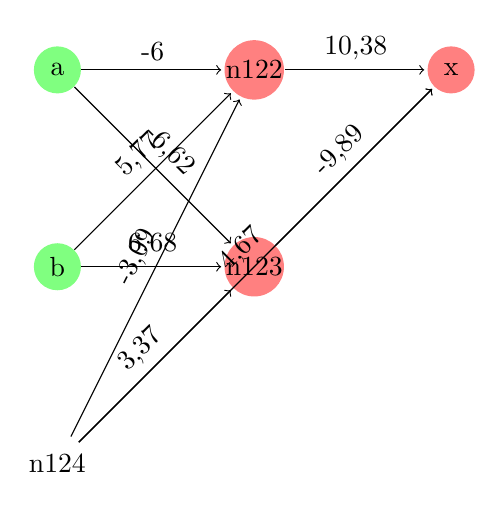
\begin{tikzpicture}[shorten >=1pt,->,draw=black!,node distance=2.5cm]
\tikzstyle{neuron}=[circle,fill=black!25,minimum size=17pt,inner sep=0pt]
\tikzstyle{constant}=[neuron, fill=white!50];
\tikzstyle{sigmoid}=[neuron, fill=red!50];
\tikzstyle{identity}=[neuron, fill=green!50];
\node [identity] (a) {a};
\node [identity,below of=a] (b) {b};
\node [constant,below of=b] (n124) {n124};
\node [sigmoid,right of=a] (n122) {n122};
\node [sigmoid,below of=n122] (n123) {n123};
\node [sigmoid,right of=n122] (x) {x};
\path[every node/.style={sloped,anchor=south,auto=false}]
(n122) edge node {10,38} (x)
(n123) edge node {-9,89} (x)
(n124) edge node {4,67} (x)
(n124) edge node {-3,09} (n122)
(n124) edge node {3,37} (n123)
(a) edge node {-6,62} (n123)
(a) edge node {-6} (n122)
(b) edge node {5,77} (n122)
(b) edge node {6,68} (n123)
;\end{tikzpicture}
\end{document}